\documentclass{beamer}

\usepackage{hyperref}

\begin{document}
\title{Automatic calculation of plane loci using Groebner bases and integration into a Dynamic Geometry System}   
\author{Michael Gerh\"auser, Alfred Wassermann} 
\date{July 24, 2010} 

\newcommand{\GEONEXT}{GEONE\kern-.06em \lower.5ex\hbox{x}\kern-.215em T}
\definecolor{GXT}{rgb}{0,0.549019608,0}
\setbeamercolor{title}{fg=GXT}
\setbeamercolor{frametitle}{fg=GXT}
\setbeamercolor{blocktitle}{fg=GXT}
\setbeamercolor{section in toc}{fg=GXT}
\usebackgroundtemplate{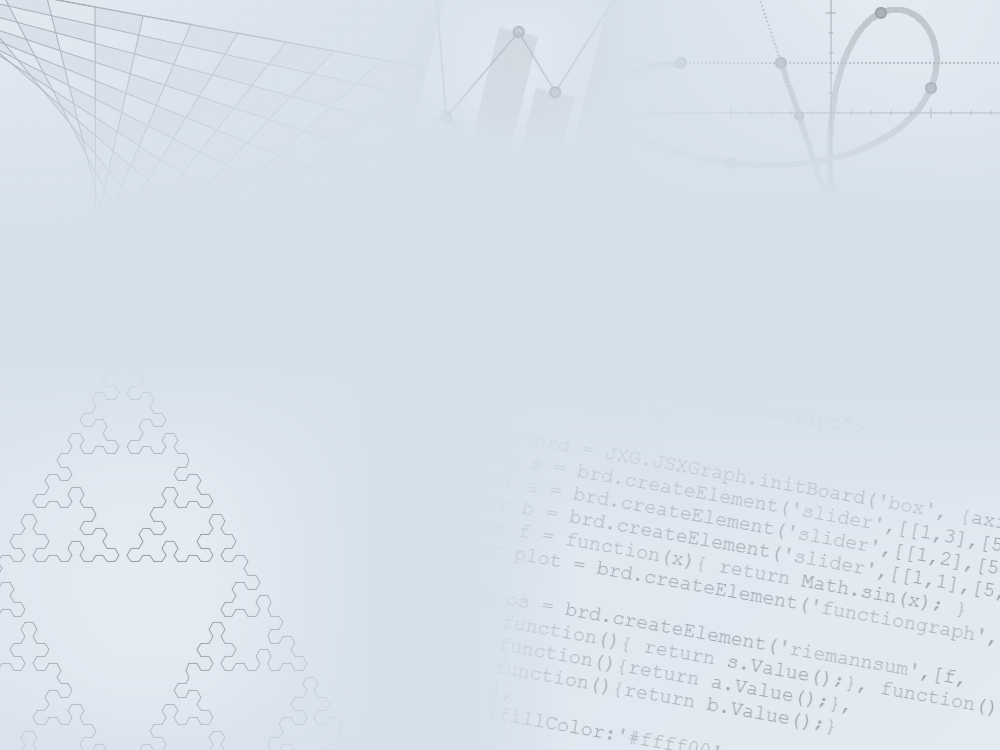
\includegraphics[width=\paperwidth]{img/background.png}}
\logo{
\includegraphics[height=0.75cm]{img/ubt.png}}
\beamertemplatenavigationsymbolsempty


\frame{\titlepage} 

\frame{\frametitle{Overview}\tableofcontents}

\section{JSXGraph - short overview} 

% JSXGraph

\frame{
  \frametitle{JSXGraph}

  \begin{block}{What is JSXGraph?}
    \begin{itemize}
      \item A library implemented in JavaScript
      \item Runs in recent versions of all major browsers
      \item No plugins required
      \item LGPL-Licensed
    \end{itemize}
  \end{block}

  \begin{block}{Features}
    \begin{itemize}
      \item Dynamic Geometry
      \item Interactive function plotting
      \item Turtle Graphics
      \item Charts
    \end{itemize}
  \end{block}
}

\frame{
  \frametitle{JSXGraph} 
  \begin{block}{Supported Hardware}
    \begin{itemize}
      \item PC (Windows, Linux, Mac)
      \item Mobile phones
      \item "Touchpads" like the Apple iPod and iPad
      \item Basically everything which runs at least one of the supported browsers
    \end{itemize}
  \end{block}
}

\frame{
  \frametitle{JSXGraph} 
  \begin{block}{Supported Browsers}
    \begin{itemize}
      \item Firefox
      \item Chrome/Chromium
      \item Safari
      \item Internet Explorer
      \item Opera
    \end{itemize}
  \end{block}
}


% Groebner bases stuff

\section{Computing plane loci using Groebner bases}

\frame{
  \frametitle{Computing plane loci using Groebner bases}

  \begin{block}{}
    \begin{itemize}
      \item Given a set of free and dependent points
\begin{center}
      \href{http://localhost/~michael/jxg/examples/adg/limacon.html}{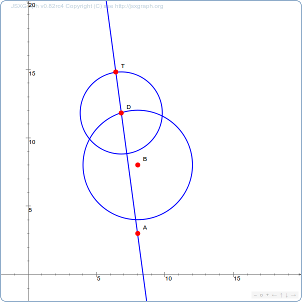
\includegraphics[width=5cm]{img/limacon-base.png}}
\end{center}
    \end{itemize} 
  \end{block}
}

\frame{
  \frametitle{Computing plane loci using Groebner bases}

  \begin{block}{}
    \begin{itemize}
      \item we first choose a coordinate system
\begin{center}
      \href{http://localhost/~michael/jxg/examples/adg/limacon.html}{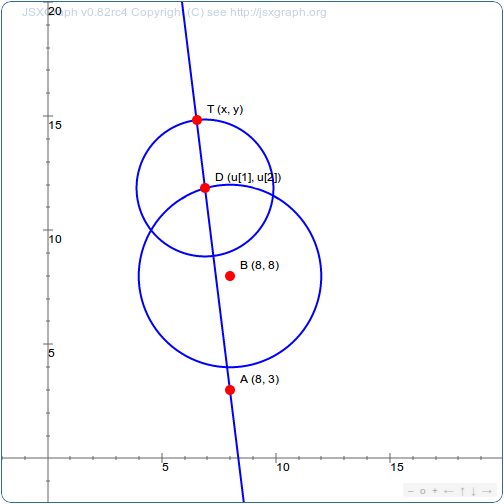
\includegraphics[width=5cm]{img/limacon-coords.png}}
\end{center}
    \end{itemize} 
  \end{block}
}

\section{Integration of this algorithm in JSXGraph}


\section{Examples}


\end{document}
